Validation of the Napali approach is intrinsically linked to validation of Makai, both with synthetic benchmarks and in-situ.
Since OPQ utilizes a custom power quality measurement device, its performance needed to be characterized prior to Makai evaluation.

\section{OPQ Box Characterization.}\label{sec:opq-box-characterization.}
A mentioned in Section~\ref{subsec:software} OPQBox generates 4 metrics in order to enable event detection.
In order to evaluate the limits of detection capabilities for each one of these metrics, an OPQBox was fed with synthetic waveform generated by the SDG1025 function generator.
By utilizing a function generator the entire device including the hardware analog front end could be evaluated.
Since the function generator is not capable of supplying $120V_{rms}$ signal, a $120mV_{rms}$ signal was fed on a low side of the OPQBox resistor divider, while the device was powered via an external 5V power supply.

\subsection{Fundamental Frequency}

Fundamental Frequency computation was evaluated by generating a 60Hz sine wave via the SDG1025 and supplying it to the OPQBox.
Calculated frequency was accumulated by analyzing the device triggering stream.
The resulting histogram is shown in Figure~\ref{fig:expdes:1}
\begin{figure}[H]
    \begin{center}
        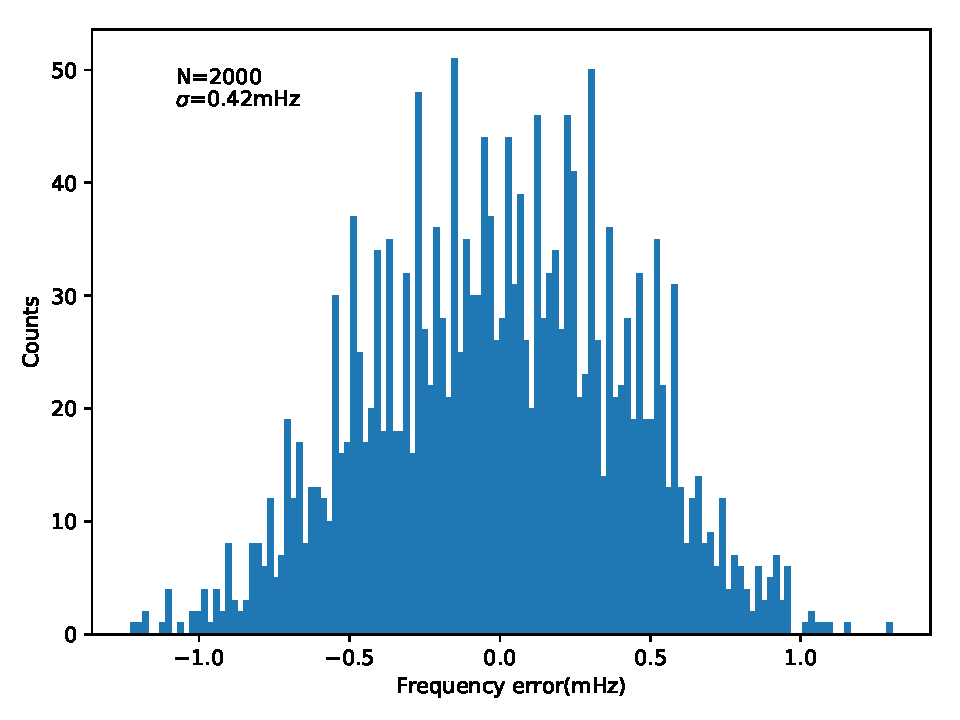
\includegraphics[width=0.6\textwidth]{img/box_eval/frequency_rms.pdf}
    \end{center}
    \caption{OPQBox frequency response.}
    \label{fig:expdes:1}
\end{figure}
As shown, the resulting distribution collected frequencies acquired over 2000s has a $\sigma=420uHz$.

\subsection{Root Mean Square Voltage}
Similarly to the fundamental frequency characterization, $V_{rms}$ calculation was evaluated by supplying the OPQBox with a 60Hz, $120mV_{rms}$ sine wave via the SDG1025.
Calculated RMS was accumulated by analyzing the device triggering stream.
The resulting histogram is shown in Figure~\ref{fig:expdes:2}

\begin{figure}[h]
    \begin{center}
        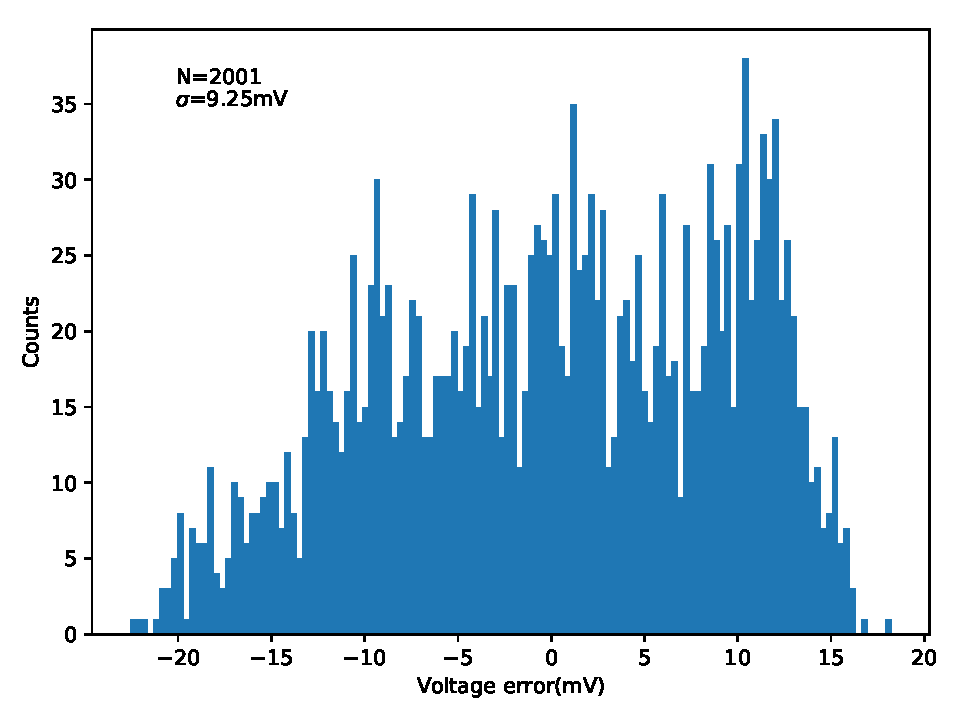
\includegraphics[width=0.6\textwidth]{img/box_eval/rms_histogram.pdf}
    \end{center}
    \caption{OPQBox $V_{rms}$ response.}
    \label{fig:expdes:2}
\end{figure}

As shown, the resulting distribution of collected $V_{rms}$ measurements, acquired over 2000s has a $\sigma=9.34mV$

\subsection{Total Harmonic Distortion}

THD performance of the OPQBox was validated by injecting a various harmonics of 60Hz superimposed onto the 60Hz, $120mV_{rms}$ sine wave into the device via the SDG1025 arbitrary waveform generation capability.
THD calculation results were acquired from the OPQBox triggering stream for analysis.
As expected resultant performance remained self-consistent across all harmonics.
Figure~\ref{fig:expdes:3} shows a histogram of the error in THD values computed form a 60Hz, $120mV_{rms}$ sinewave superimposed with a 240Hz $1.2mV_{rms}$ sine wave.
This measurement is equivalent to $1\%$ THD at the $4^{th}$ harmonic.

\begin{figure}[h]
    \begin{center}
        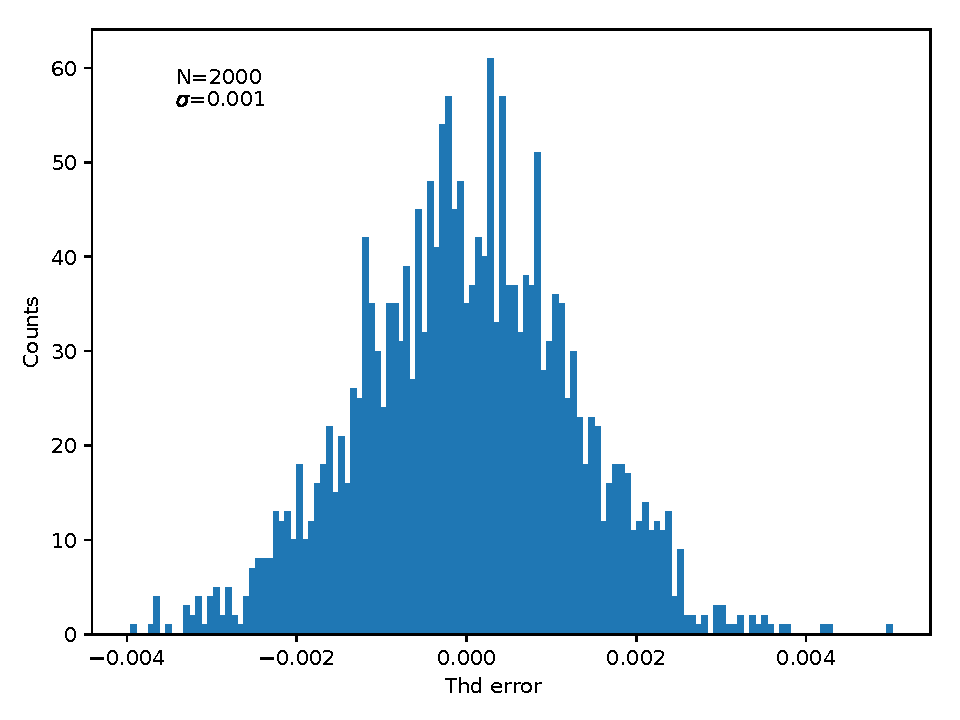
\includegraphics[width=0.6\textwidth]{img/box_eval/thd_rms.pdf}
    \end{center}
    \caption{OPQBox THD response.}
    \label{fig:expdes:3}
\end{figure}

As shown, the resulting distribution of collected THD measurements, acquired over 2000s has a $\sigma=0.001\%$.

\subsection{Transient Detection}

Transient detection performance was evaluated by injecting a transient superimposed onto the 60Hz, $120mV_{rms}$ sine wave into the device via the SDG1025 arbitrary function generation capability.
Transient detection results were acquired by capturing and analyzing the device triggering stream.
Transients of various shapes and magnitudes were tested.

\begin{figure}[h]
    \centering
    \begin{subfigure}{.5\textwidth}
        \centering
        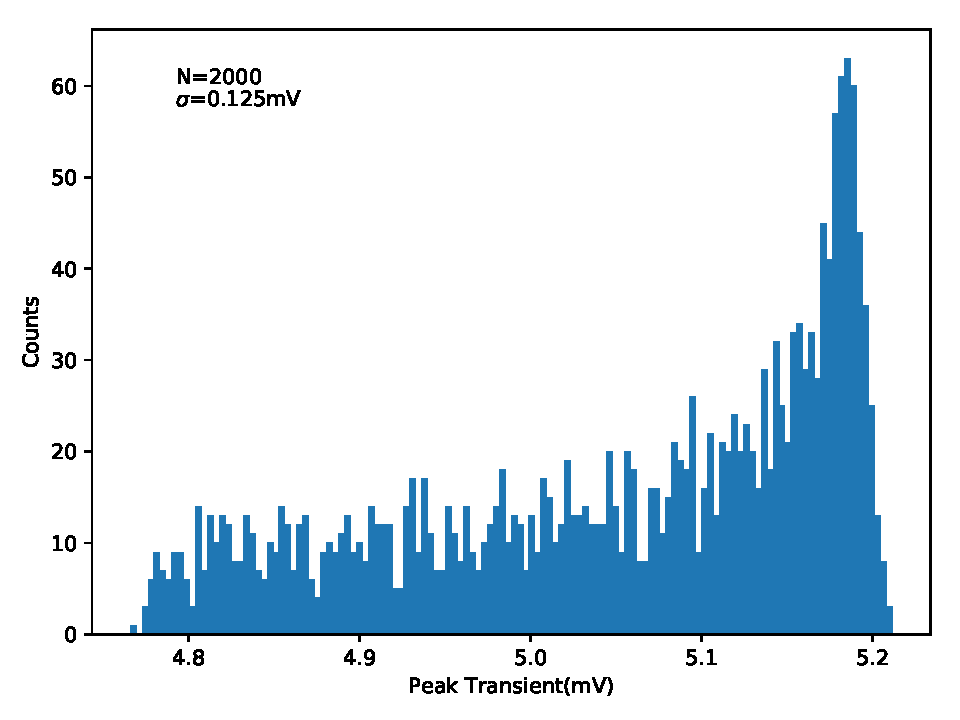
\includegraphics[width=0.9\linewidth]{img/box_eval/5v_transient_rms.pdf}
        \caption{}
        \label{fig:expdes:4:1}
    \end{subfigure}%
    \begin{subfigure}{.5\textwidth}
        \centering
        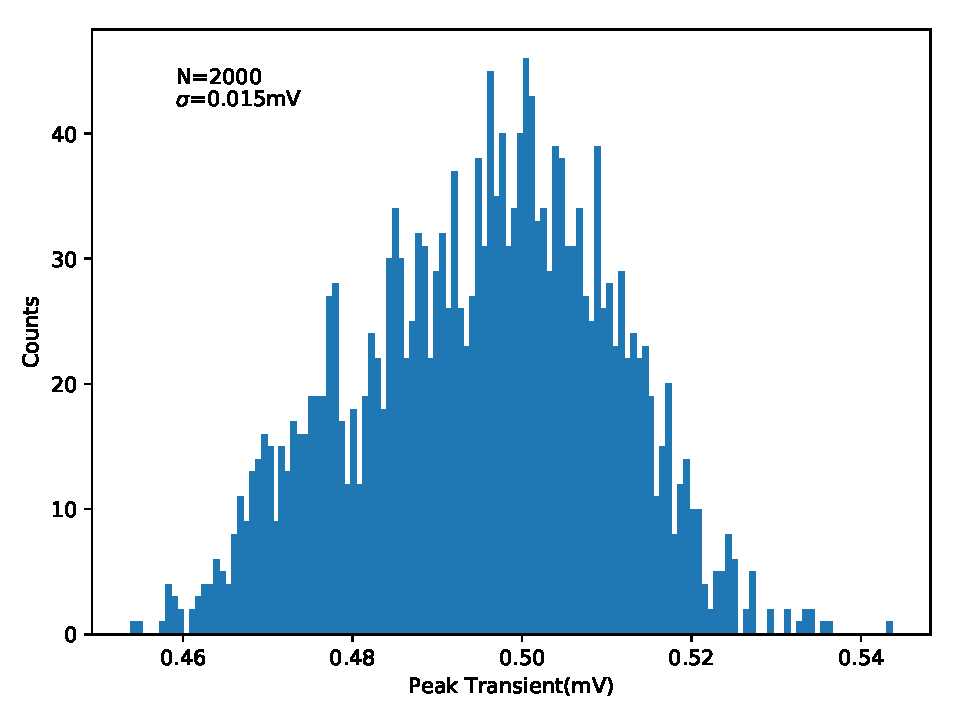
\includegraphics[width=0.9\linewidth]{img/box_eval/0p5v_transient_rms.pdf}
        \caption{}
        \label{fig:expdes:4:2}
    \end{subfigure}
    \caption{Transient detection metric with a 5V transient(a), and 0.5V transient(b)}
    \label{fig:expdes:4}
\end{figure}

Figure~\ref{fig:expdes:4} shows the resultant transient detection metric for two transients.
The shape of the transient is the same and is shown in Figure~\ref{fig:opq:8:3}.
Interestingly, in case of a 0.5V transient the metric results in a much tighter distribution with $\sigma =0.015V$, while in the case of
a 5V transient the distribution exhibits a lower sideband tail.
Since the transient is injected in a random position in the cycle, and the sampling rate of the DG1025 is significantly higher then sampling rate of the OPQBox(25Msps vs 12Ksps), the peak of the transient will sometimes fall in between the consecutive samples of the OPQBox.
In the $0.5V$ transient case this effect is alleviated, since the transient is so small.
Regardless, the result shown in Figure~\ref{fig:expdes:4:2} is presented only as a synthetic benchmark, since OPQBox is expected to operate in an environment with THD larger then $0.4\%$ at $>400Hz$ required to detect a $0.5V$ transient.
As such, the figure of $\sigma=0.125V$ should be considered valid for the OPQBox transient detection capability.
Since this metric is only used in transient detection and not characterization, it was found to be sufficient.

\section{Napali Validation}\label{sec:napali-validation.}
Napali method was validated using simulation, synthetic data with the device-in-loop, and in-situ during the deployment.
The main tunable parameter in the napali is the $\alpha$ coefficient used in the low pass filter as shown in Equation \ref{eq:iir_mean}.
This parameter determines the memory of the lowpass filter used in the calculation of the mean and the standard deviation of metrics from OPQBox data stream.
These statistics are in turn used during the Napali triggering process to locate sub-threshold gridwide events.

\subsection{Selection of $\alpha$ parameter}\label{subsec:selectrion-ofparameter}
Smaller $\alpha$ parameter corresponds to a longer memory in the low pass filter as shown in Equation \ref{eq:iir_alpha}.
This is further visualized in Figure \ref{fig:expdes:5}.
In particular this Figures \ref{fig:expdes:5:1} and \ref{fig:expdes:5:2} show the response of the IIR low pass filter to the simulated frequency measurements.
The dashed red line represents the frequency measurement, solid red line represents the filtered mean, and the blue line represents the standard diviation.
Figures \ref{fig:expdes:5:1} shows the filter response for $\alpha = 0.5$ or $T_{memory} \approx 10s $.
As evident from the plot, the mean and the standard deviation quickly recover from the transient are return to the nominal values.
Furthermore, the mean is closely tracking the random fluctuations present in the measurement.
Figures \ref{fig:expdes:5:1} shows the filter response for $\alpha = 0.05$ or $T_{memory} \approx 123s $.
While the stimuli remains the same, it takes significantly longer the statistics to recover.
Additionally, the mean no longer tracks the frequency fluctuations present in the simulated data.

\begin{figure}[h]
    \centering
    \begin{subfigure}{0.9\textwidth}
        \centering
        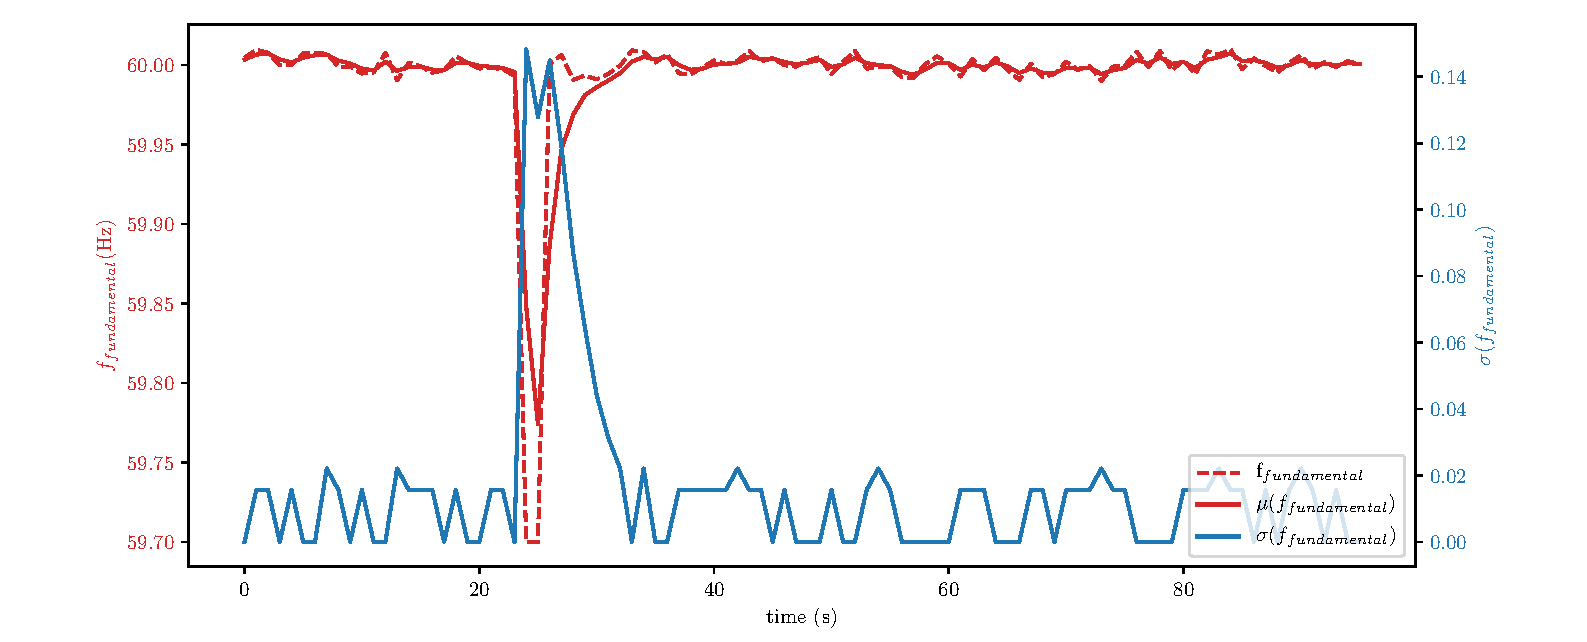
\includegraphics[width=1\linewidth]{img/napali_eval/Napali_response_freq_05.pdf}
        \caption{}
        \label{fig:expdes:5:1}
    \end{subfigure}%

    \begin{subfigure}{0.9\textwidth}
        \centering
        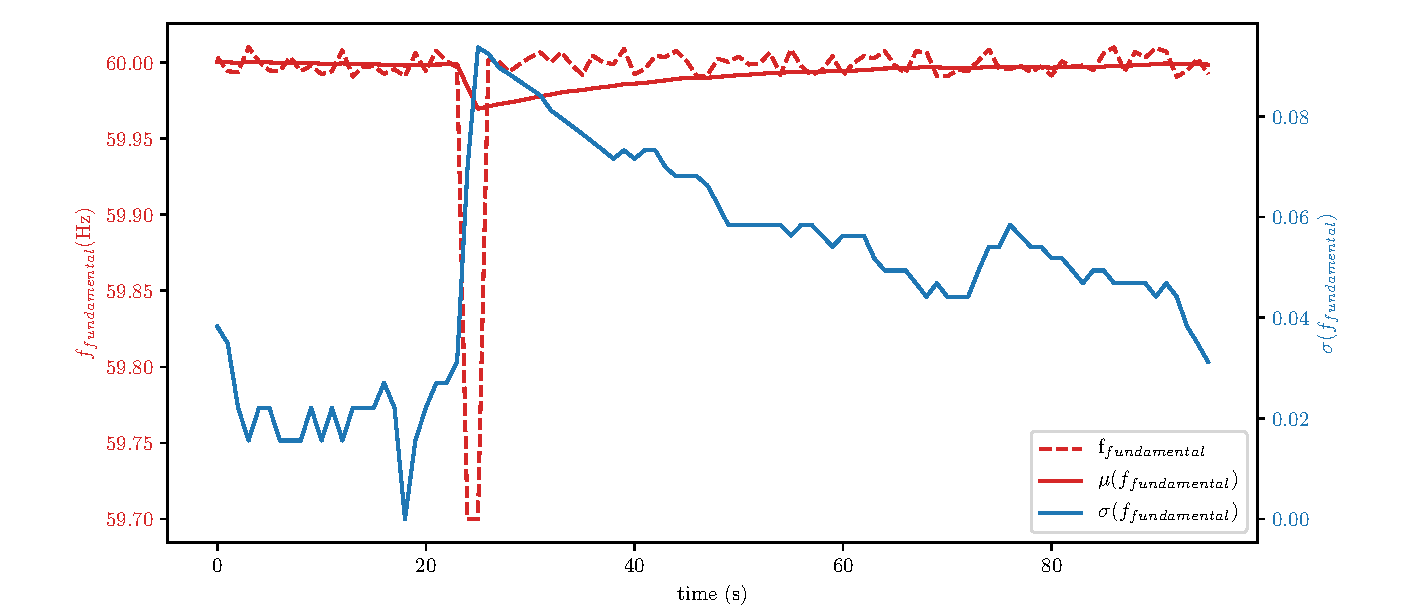
\includegraphics[width=1\linewidth]{img/napali_eval/Napali_response_freq_005.pdf}
        \caption{}
        \label{fig:expdes:5:2}
    \end{subfigure}
    \caption{$\mu$ and $\sigma$ behaviour with a)$\alpha = 0.5$ and b)$\alpha=0.05$}
    \label{fig:expdes:5}
\end{figure}

Picking the $\alpha$ parameter for Napali is extremely domain specific, as it depends on the frequency content of the triggering stream.
Intuitively, the $T_{memory}$ parameter needs to be long enough to adjust to gradual changes in the triggering stream for the mean calculation,
and dampen the standard deviation for detection of multiple consecutive outliers.
In addition, it needs to be short enough to be converge on the mean and the standard deviation during a step-like transition in the triggering stream.

Luckily, in the Power Quality domain the Napali $\alpha$ selection is fairly forgiving.
This is demonstrated in Figure \ref{fig:expdes:6}.
This graph represents the amount of time that Napali considered one of the metrics to be outside of the $3\sigma$ of the mean for various values of $\alpha$.
The triggering stream used to generate these values was captured over 24 hours by one of the OPQBoxes deployed on the University of Hawaii campus.
All devices deployed thus far have followed a similar pattern.
With $200s <T_{memory} < 2Hr$ the triggering stream resulted in similar behaviour, with the system correctly marking all potential sub-threshold events.
At $T_{memory} \approx 500s$, system quickly recovered from large jumps in the triggering stream, however it marked a significant number of small deviations ($\Delta_{f}>0.01Hz$, $\Delta_{v}> 0.1V$\ldots etc) as outside $3\sigma$, and thus candidates for sub-threshold events.
At $T_{memory} \approx 2Hr$, system took  significant amount of time to recover from large jumps in triggering metrics, thus marking the metric as outside of $3\sigma$ for many tens of minutes.
Furthermore, some of the larger anomalous measurements ($\Delta_{f}>0.05Hz$, $\Delta_{v}> 2V$\ldots etc) were no longer flagged as sub-threshold candidates.
Outside of the two extremes, the system behaviour was quite similar.
During all of the deployments the OPQ system was operating with:
\begin{equation}\label{eq:opq_alpha}
\begin{aligned}
    \alpha = 0.005
\end{aligned}
\end{equation}


Which corresponds to the $T_{memory} \approx 21$ minutes.
Thresholds which initiate the event are shown in Table \ref{tbl:opq:thresholds}.

\begin{figure}[h]
    \centering
        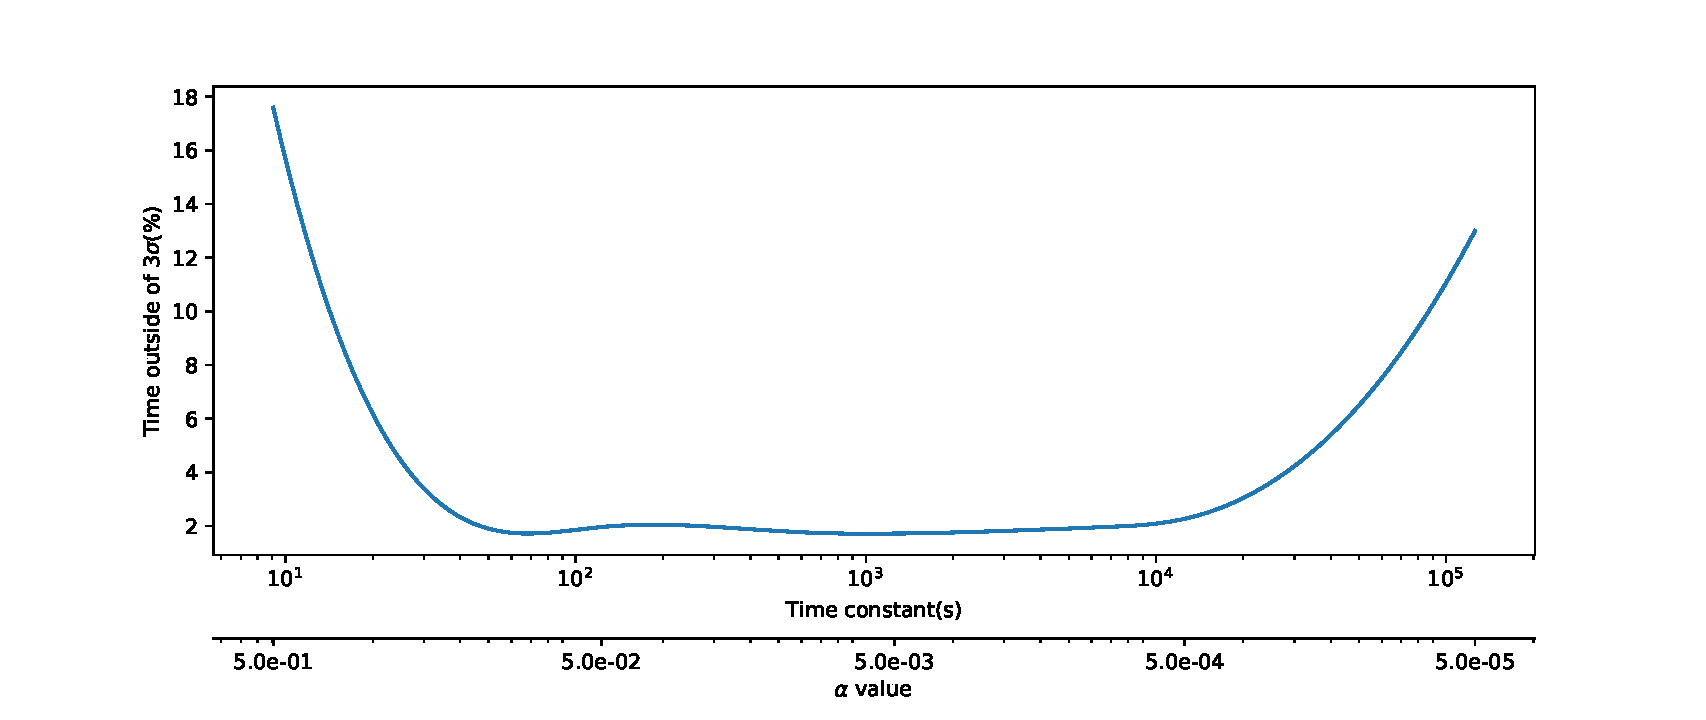
\includegraphics[width=1\linewidth]{img/napali_eval/a_selection.pdf}
    \caption{Amount of time a metric spends outside of the $3\sigma$ for various values of $\alpha$}
    \label{fig:expdes:6}
\end{figure}

The effect of the of selecting alpha as shown in Equation \ref{eq:opq_alpha} can be observed in Figure \ref{fig:expdes:7}.
This figure shows interesting features form the same dataset that was used to produce Figure \ref{fig:expdes:6}.
Blue traces show metrics that exhibit anomalous behaviour, while red indicates that Napali has flagged this temporal region as a sub-threshold event candidate.
Figure \ref{fig:expdes:7:1} shows a frequency fluctuation which nearly passes the threshold of $60.1Hz$ which would mark it as a full fledged event.
Instead, Napali marked almost the entirety of the fluctuation as a potential sub-threshold event, as shown by the red trace.
Figure \ref{fig:expdes:7:2} shows a step in the total harmonic distortion metric, similar to the one shown in Figure \ref{fig:opq:7} at the 6am mark.
In this case the metric in question abruptly changed to a new mean, requiring a fairly slow $\alpha$ coefficient to catch up over 3 minutes.
While it may seem wasteful to mark large temporal regions following an abrupt jump as candidates for sub-threshold event, it is important to note that:
\begin{enumerate}
    \item Making the $\alpha$ parameter smaller does not benefit the false positive rate as shown in Figure \ref{fig:expdes:6}.
    \item In-situ there is no way to tell if an abrupt shift is a switch to a new steady state, or if the metric will recover to a previous mean.
\end{enumerate}
It is important to remember than Napali is not meant to have a low false positive rate.
Instead, a system like OPQ Mauka can use all available information, including the raw data, to determine if an event is gridwide or not with much higher confidence.
The main goal of Napali is to have an extremely low rate of false negatives.
Figure \ref{fig:expdes:7:3} is on a different timescale from Figures \ref{fig:expdes:7:2} and \ref{fig:expdes:7:1}.
This is done in order to include several potential sub-threshold events into a common chart.
Five temporal regions during the the 3 Hrs are marked by Napali as potential sub-threshold events.
\begin{figure}[h]
    \centering
    \begin{subfigure}{0.5\textwidth}
        \centering
        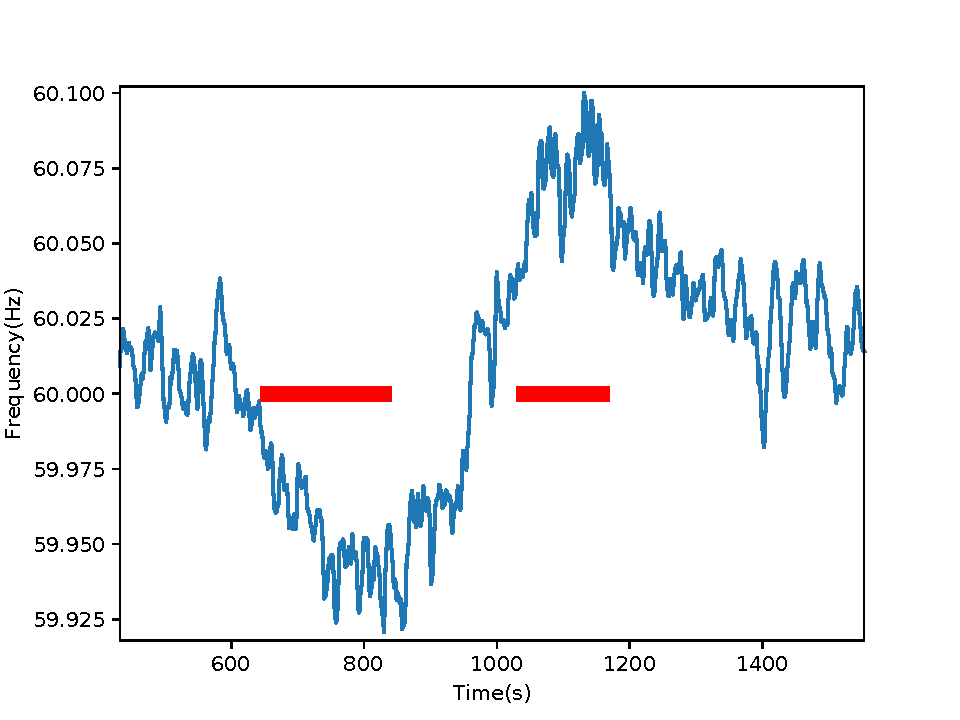
\includegraphics[width=1\linewidth]{img/napali_eval/napali_live_f.pdf}
        \caption{}
        \label{fig:expdes:7:1}
    \end{subfigure}%
    \begin{subfigure}{0.5\textwidth}
        \centering
        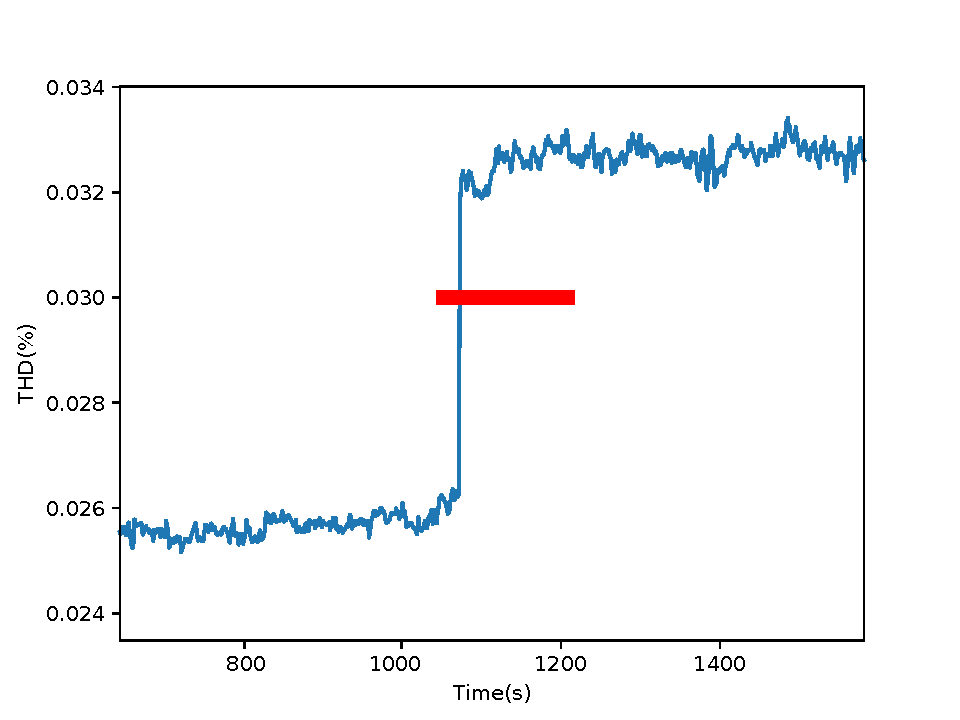
\includegraphics[width=1\linewidth]{img/napali_eval/napali_live_thd.pdf}
        \caption{}
        \label{fig:expdes:7:2}
    \end{subfigure}

    \begin{subfigure}{0.5\textwidth}
        \centering
        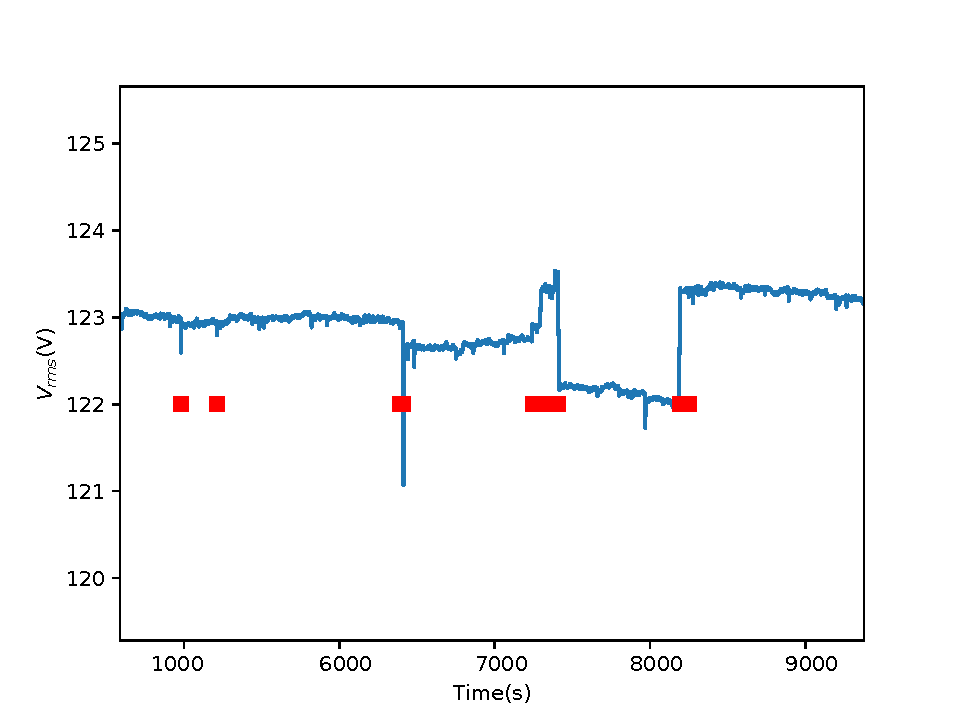
\includegraphics[width=1\linewidth]{img/napali_eval/napali_live_rms.pdf}
        \caption{}
        \label{fig:expdes:7:3}
    \end{subfigure}%
    \begin{subfigure}{0.5\textwidth}
        \centering
        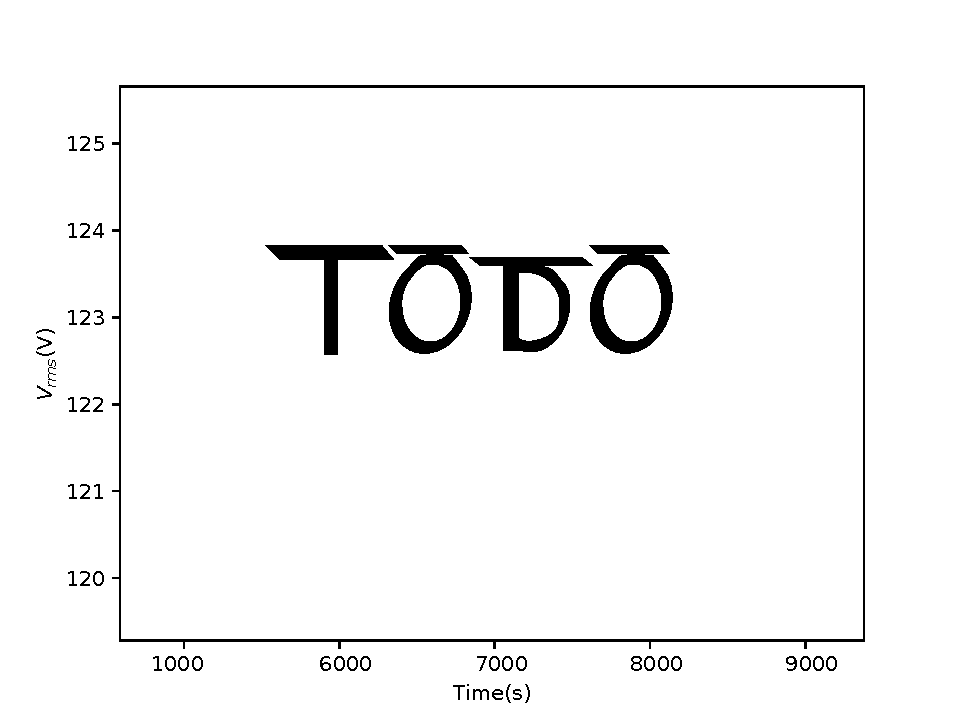
\includegraphics[width=1\linewidth]{img/napali_eval/napali_live_trans.pdf}
        \caption{}
        \label{fig:expdes:7:4}
    \end{subfigure}

    \caption{Potential sub-threshold events for a) $f_{fundamental}$, b)$THD$, c)$V_{rms}$ and d)$Trans$.
    Red boxes indicate that Napali picked these temporal windows as a potential sub-threshold event.}
    \label{fig:expdes:7}
\end{figure}

\subsection{Sub-Threshold Event Detection}

\clearpage

\clearpage

\section{Stop Reading here.}\label{sec:stop-reading.}
In order to validate the OPQ system as a whole, it will be deployed across the University of Hawaii Manoa campus (UH).
This location is ideal because it is a relatively isolated microgrid connected to the Oahu powergrid only via a single 46kV feeder as shown in Figure~\ref{expdes:fig:1}.
Another advantage of the UH campus is the high number of smart meters deployed across various levels of the power delivery infrastructure.
While these meters are mainly geared towards monitoring power consumption they do have some power quality monitoring capabilities.
Data provided from these meters can be used in two distinct applications.
First of all, this data can be used to pinpoint the sections of the University of Hawaii power grid which experience a higher likelihood of power quality disturbances.
These portions of the grid will have a higher spacial density of OPQ Boxes.
Secondly, data from the campus deployed meters can be used as ground truth for comparison against the measurements, and analysis performed by the OPQ project.
The location of smart meters in the grid topology is shown in figure~\ref{expdes:fig:1} as the $M$ nodes.
As evident by the meter location none of them are monitoring the consumer level power and mainly focus on the higher voltage power delivery.
This placement is evidenced from the smart meter role as a consumption monitor, and thus the deployment of the OPQ Boxes at the residential level will compliment the current power quality monitoring capabilities without introducing redundancies.
Finally, the University of Hawaii power grid is supplying a highly diverse infrastructure.
Beyond the traditional residential equipment such as computers and consumer grade electronics, the UH power grid powers scientific and laboratory equipment, machine shops, and server farms.
All of these elements have varying requirements/tolerances for power quality anomalies as well as different levels of power quality ``pollution''.
Furthermore, some of the electricity consumers in the UH campus are entirely unique.
For example, the free electron laser located in the Watanabe Hall is one of the only free electron lasers in the world, and the impact/sensitivity of power quality on the instrument are completely unstudied.
\begin{figure}[h]
	\centering
	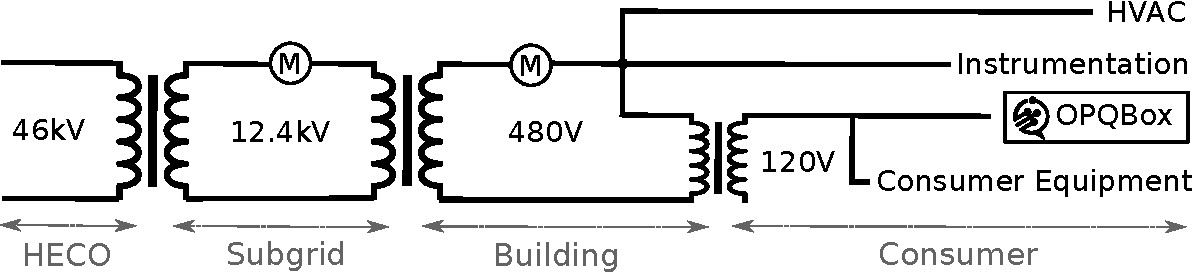
\includegraphics[width=1\linewidth]{img/uh-grid.pdf}	
	\caption{University of Hawaii at Manoa power delivery infrastructure.}
	\label{expdes:fig:1}
\end{figure}

There are 74 smart meters deployed across the UH campus.
These meters measure the fundamental frequency $V_{rms}$, power consumption, reactive power, and power factor.
Data from these meters will be cross-referenced with the Napali detection system in order to ascertain it's benefits.
Validations of the benefits of the Napali framework will follow the framework described in Section~\ref{intro:sec:claim}.
Here we examine the analysis required to complete each claim in detail.

\subsection{Napali Bandwidth usage} \label{iexp:sec:band}
In order to analytically compute the bandwidth savings of the Napali compared to a system which sends all the data to the sink, I will keep track of the amount of bandwidth the Napali monitoring system consumed during its deployment on UH campus.
This will in turn be compared to the bandwidth required by the OPQ Boxes if they were sending the entirety of the data to the sink, and establish the bandwidth efficiency of the Napali framework.
In order to monitor the bandwidth of the system in-situ, an iptables bandwidth accounting will be enabled on the sink node.
With the accounting enabled, I will be able to extract the exact amount of bytes transfered by the Napali framework during the deployment period.
Since the sampling rate of the OPQ Box is well characterized, and the number of OPQ Boxes is fixed, it is trivial to calculate the amount of raw data generated by the OPQ network during any time period.
In order to make this comparison fair, the raw data bandwidth will be scaled by the compression ratio of the state of the art compression algorithm specifically designed for power quality measurements.\cite{zhang2009new}

Operating at 12kSps, OPQ Box produces raw data at 24KB/s.
With state of the art compression operating at 90\% compression ratio and a 5\% overhead of TCP/IP and meta-data, one can expect a ~3KB/s stream of raw data for each OPQ box if it were to send the entirety of it to the sink.
In synthetic experiments, under steady state conditions, OPQ Box consumes 0.5KB/s of bandwidth sending metrics to the Makai.
However, this figure does not take into account sending the raw data samples in case an event is detected.
The result of bandwidth consumption evaluation will provide a comparison of the bandwidth consumption by Napali methodology of sending metrics and temporal raw data windows of interest compared to sending the entirety of raw data to the sink.

\subsection{Sink processing requirement under the Napali Framework} \label{iexp:sec:scale}
In order to evaluate the scalability of the sink node under the Napali framework, synthetic data containing a small amount of distributed events will be injected into the Makai triggering system.
While the synthetic data for a single point PQ disturbance is easily generated, distributed PQ event generation is not well understood.
However there is some literature concerning power fault propagation and localization.~\cite{parsons1998direction}~\cite{polajvzer2017evaluation} The main takeaway from these authors is the energy and amplitude of the event diminishes with electrical distance from the source.
As such, by generating a single point PQ event as described in~\cite{kumar2015power}\cite{tan2013simulation}, and linearly scaling it based on the simulated electrical distance from the source, a distributed PQ event ensemble can be generated.
These events will be ran through the simulated OPQ Box DSP stack and the extracted metrics will be propagated to the Makai aggregation sink.
The number of simulated OPQ Box devices that can be supported on a single node will be recorded, and will provide the baseline for the Makai sink node capabilities.
Next, the same dataset will be processed on the same node using simulated OPQ Box software stacks.
The amount of concurrent processes which are able to keep up with the targeted sampling rate of $12kS/s$ will be determined and recorded, and compared to the amount of devices which can be supported by Makai.

The result of this evaluation will provide a scalability metric for the Napai framework for a single sink node.
There are independent metrics which will be presented.
First, the number of OPQ Boxes which can reliably send metrics to a single Makai instance for processing will be established.
This number is expected to be quite high since the bandwidth and computational requirements for processing the triggering stream are quite low.
Second, the number of OPQ Boxes, that can experience and reliably send an event to Makai at the same time will be established.
The bandwidth requirement for raw data acquisition is significantly higher then the triggering stream, however there is no computation involved in storing raw data frames.
Both of these metrics will be compared to the scalability of performing the entirety of processing on the sink node.

\subsection{Effects of latency in the Napali framework} \label{iexp:sec:lat}
The latency of Napali triggering system has a significant impact on its ability to read out complete raw data events.
Using generated distributed events as a baseline, I will be able to tune the threshold and temporal requirements for Makai detection algorithms.
Furthermore, temporal, spacial, and amplitude noise will be injected into the generated datasets, to simulate various uncertainties with regards to data collection, such as local noise, and NTP offset errors.
Taking into the account the detection latency of Makai, if some of the requested data is no longer available on the OPQ Box, only a partial time window will be returned.
These events will be marked as incomplete and their fraction as compared to the total number of events recorded will be used to establish the latency tolerance of the Napali framework.
Synthetic benchmarks will be carried out to establish the latency that the Napali system can incur without losing a portion of the event.
Since this is highly dependent on the amount of storage allocated for the RDRB, these experiments will be carried out with various RDRB settings.

Because OPQ Boxes operate using public University of Hawaii WIFI, the latency figures for data transmission are expected to be very dynamic.
In situations with large network contention, greater then 100ms one way packet latency can be expected.
This latency is exacerbated since at least three separate communication steps are required before raw data is received by Makai.
First the metric has to be sent to Makai, next if Makai detects an event, a data request needs to be sent to the affected boxes.
Finally boxes will forward raw data to the Makai sink.
I expect that with RDRB capacity of storing 5 seconds of raw data, no raw data events of 1s or shorter will be missed.
This figure allows for 1 second of transfer latency, 3 seconds of Makai analysis latency, and leaves 1 second of data in RDRB for readout.
However, these figures can only be validated in a real world situations.

\subsection{Temporal locality triggering of the Napali framework} \label{iexp:sec:loc}
Once the OPQ Box is fully validated and the Makai detection thresholds are tuned using synthetic datasets, the Napali system will be fully deployed at the University of Hawaii at Manoa.
 Every time the Napali detects an event, both OPQ Boxes and building meters will be queried for data.
 While it may be unfeasible to query raw data from the UH metering infrastructure, metrics are readily available.
 This data will be used to ascertain the proportion of false positive events detected by Napali.
 Additionally, the internal single point fault detection mechanism of the UH power meters will be used in conjunction with the events detected by Napali to measure the rate of false negative events.
 Both the false negative and false positive measurements will be used to ascertain the detection efficient of the Napali framework.
 This analysis will also include an evaluation  of Napali's ability to reject single point anomalies.
 For a portion of OPQ deployment, every event triggered by a single device will be captured.
 These events will be analyzed in order to determine if a gridwide anomaly was incorrectly classified as a single point disturbance.

The goal of Napali is not to to provide a zero false positive rate.
Once raw data is stored, higher level processing can further filter and classify it using more computationally expensive techniques.
As long as the bandwidth consumption of Napali compares favorably to sending the entirety of raw data to the sink, any rate of false positives can be tolerated.
False negatives on the other hand are the primary metric subject to optimization.
Ideally a zero rate of false positives would be expected, however as with any real-world system I do not expect that to be the case.
This evaluation will determine the triggering efficiency of the Napali framework when compared to the detection ability of a commercially available system.

\subsection{Sub-threshold Data Acquisition} \label{iexp:sec:sub}
The Napali methodology will be compared with the single point anomaly detection approach.
In order to do that I will compare the extent to which sub-threshold events are missed by the UH metering infrastructure.
In a large distributed event, if a portion of events are not detected by the UH meter's single point detection, but picked up by the Napali framework, these events will be flagged and analyzed for their merit.
This will in turn provide a metric of distributed detection ability of the Napali framework compared to commercial system.
Furthermore, for a portion of the deployment the triggering stream from the OPQ Boxes will be stored along with the acquired raw data.
The triggering stream can be used to compute which fraction of devices would have self triggered if operating autonomously.
This will provide the baseline for sub-threshold triggering efficiency of the Napali system, with respect to the single point detection ability of the OPQ Box.

This evaluation will compare Napali performance to the single point detection mechanisms currently in deployment.
I expect that Napali will outperform these strategies, and provide a more complete picture of gridwide anomalies as they propagate through the UH power grid.
It is possible that no sub-threshold events will be recorded during the UH deployment.
UH campus is quite small, perhaps too small for an anomaly in one building not to impact the rest of campus.
In this case the sub-threshold data acquisition will remain an open topic for future work and a larger geographical deployment.
Regardless, as long as I am be able to validate the single point anomaly rejection ability of Napali as described in Section~\ref{iexp:sec:loc}, I will be able to conclude that Napali has a distinct advantage over single point detection methods.
Single point anomalies are not important in smart grid monitoring, since they originate from the consumers side of the meter, and should be ignored.
In fact, recording these events may be detrimental to the privacy of the end-user, since it may give clues on their activities as shown in Figure~\ref{intro:fig:1} a and b.
However since privacy implication of power quality monitoring are outside the scope of this project, this study will remain as a point of future work.
